\documentclass{article}
\usepackage{graphicx} % Required for inserting images
\usepackage{url}
\usepackage{hyperref}

\title{Building DTSA-II Microanalysis Tools}
\author{Nicholas Ritchie}
\date{\today}

\begin{document}

\maketitle

\section{Introduction}
This document describes the procedures to build and deploy NIST DTSA-II, NIST Graf, NIST Glass Database, the Relocation application and SEMantics.

\begin{description}
    \item[Build] Reconstruct the applications from the Java source code and other build artifacts.
    \item[Deploy] Build installation applications which can be distributed to users to make the necessary changes to their systems to run the programs.
\end{description}

\subsection{Core Java Code}
The DTSA-II tool set consists of multiple different Java libraries and Java applications.  This code is typically compiled using a Java Development Tool (JDK) kit. As of January 2025, the current long-term supported release of the JDK is version 21 and this is used to compile the entire project.

\begin{description}
    \item[EPQ] The Electron Probe Quantification library.  A Java library that provides the basic X-ray microanalysis algorithms used by DTSA-II, Graf and SEMantics.
    \item[FastQuant] A Java library that provides a very fast but less accurate mechanism for extracting k-ratios from X-ray spectra.
    \item[DTSA-II] `Power-tools for X-ray Microanalysis` The core application in the NIST microanalysis suite.
    \item[Graf] A X-ray microanalysis application focused on processing automated particle analysis data sets.
    \item[Relocation] A stand-alone application for perform coordinate transformations for samples moved between instruments.
    \item[Glass Database] A standalone application for working with NIST K-glasses.
    \item[SEMantics] A library that extends DTSA-II to provide TESCAN instrument control functionality to implement image, spectrum and particle analysis data acquisition.
    \item[JythonGUI] A standalone application for scripting the EPQ library.  Primarily used by John Villarubia and his collaborators.
\end{description}

Each of these libraries and applications is a separate code-base.  The code bases are either maintained on \href{https://github.com/}{GitHub} under the \href{https://github.com/usnistgov}{usnistgov} organization or on NIST's \href{https://gitlab.nist.gov}{GitLab}.  See Table \ref{tab:code_urls} for the locations of the canonical code-bases.

\subsection{Security}
The core projects (DTSA-II and EPQ) are on GitHub and are accessible to anyone (NIST and the general public) as is the nature of "Open Source" software.  While it is possible for anyone to \href{https://docs.github.com/en/pull-requests/collaborating-with-pull-requests/working-with-forks/fork-a-repo}{fork} a project and make changes to the "forked" project.  Currently, the only person with rights to modify the base DTSA-II and EPQ projects is Nicholas Ritchie.  Others may suggest modifications through the \href{https://github.blog/developer-skills/github-education/beginners-guide-to-github-merging-a-pull-request/}{Pull Request} process.

More sensitive projects are maintained on NIST's GitLab.  NIST's GitLab is accessible only to NIST badge holders who have been given permission to join.

\begin{table}[h!]
    \centering
    \begin{tabular}{p{96pt}p{225pt}}
        \emph{Code-base} & \emph{Comment} \\
        \href{https://github.com/usnistgov/DTSA-II}{DTSA-II} & Managed by USNISTGOV organization \\
        \href{https://github.com/usnistgov/EPQ}{EPQ} & Managed by USNISTGOV organization \\
        \href{https://gitlab.nist.gov/gitlab/nritchie/graf}{Graf} & On the NIST GitLab site.  Graf was originally developed for OA use. \\
        \href{https://gitlab.nist.gov/gitlab/nritchie/nist-glass-database}{Glass Database} & On the NIST GitLab site.  The NIST glass database is of little use to people outside of NIST who don't have access to NIST K-glasses. \\
        \href{https://gitlab.nist.gov/gitlab/nritchie/semantics}{SEMantics} & On the NIST GitLab site.  SEMantics was developed for OA use. \\
        \href{https://github.com/usnistgov/EPQ}{Relocation} & Include as part of \href{https://github.com/usnistgov/EPQ}{EPQ} \\
        \href{https://gitlab.nist.gov/gitlab/nritchie/fastquant}{FastQuant} & On the NIST GitLab site.  FastQuant implements algorithms that were considered proprietary at the time of implementation. They are no longer considered proprietary. \\
    \end{tabular}
    \caption{The name and URL at which the canonical version of each code-base can be found.}
    \label{tab:code_urls}
\end{table}

\subsection{Building Everything}
To facilitate the build process, there is a single file (`Installer/build\_install.bat`) located within the DTSA-II code-base that, when configured correctly, will build all the applications in the DTSA-II tool set.  `build\_install.bat` is executable from the Windows command line.  It will configure and rebuild all the Java source code, rebuild the Windows .exe files which make starting the applications easier on Window and build three different Java executable install programs.

\begin{description}
    \item[Base] Installs the DTSA-II (required), Relocation (optional) and Glass Database (optional) tools.  Compatible with Apple OS, Windows and Linux.  Requires a Java Runtime Environment 21 or above to execute the tools.
    \item[Base With JRE] Same tools as Base but adds a Windows compatible Java Runtime Environment so the user does not need to install one separately.
    \item[Full] Adds Graf, SEMantics and FastQuant to the `Base with JRE` install.  This installer is designed only for distribution to NIST and our OA partners.
\end{description}

\begin{figure}
    \centering
    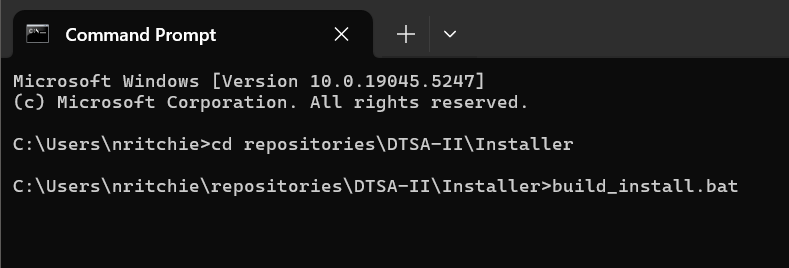
\includegraphics[width=0.5\linewidth]{CmdPmt_build_install.bat.png}
    \caption{Running the batch file from the command line.}
    \label{fig:batch}
\end{figure}

Towards the top of the `build\_install.bat` file, a number of environmental variables are configured. These variable control various aspects of the build. The `D2V`, `NUM\_VER` and `NAME\_VER` variables are used to track version information.  `D2V` contains the build date and `NUM\_VER` contains a `major.minor.build` version number that is incremented each fresh build.  The `NAME\_VER` is updated alphabetically approximately once-per-year when a major update is performed.  The `minor` version number is updated when the `NAME\_VER` is updated and the `build` version is reset to one.  All `.jar` filename include the `NUM\_VER` to ensure that the libraries match each other.

Below the version information is a set of environmental variables that point to the locations of various important build directories.  These are currently configured to build the project on the NIST laptop G909897.  They will need to be updated to reflect the location of build tools on whatever system is used to rebuild the project.

\section{Software Development Tools}
\subsection{Java Development Kit (JDK)}
All the applications have been developed in Java and can be compiled with \href{https://adoptium.net/temurin/releases/?os=windows&arch=x64&package=jdk}{JDK 21}.  Java applications can be compiled on any Java supporting operating system.  The resulting '.jar' files can be deployed on any operating system supporting the Java Runtime Environment (JRE). NIST DTSA-II and its sibling applications have all been developed on a Microsoft Windows system.  However, they are known to work on Apple OS and Linux (Fedora).

\subsection{Git}
\href{https://git-scm.com/}{Git} is a distributed version control system used to administer the source code associated with each application.  While it is possible to download the source code directly from the remote repository (usually as a compressed archive), it is generally better to work with a Git tool to maintain synchronization between local and remote repositories.
\begin{description}
    \item[\href{https://git-scm.com/}{Command line}] This command line tools allow you to synchronize source code stored in a remote repository with a repository on your local system.  Git can be hard to understand at first.  A thorough introduction is available here: \url{https://git-scm.com/book/en/v2}
    \item[\href{https://www.gitkraken.com/}{GitKraken GUI}] This graphical user interface provides an easier to use mechanism to synchronize a remote repository with a local repository.
    \item[Alternative GUIs] An extensive list of alternative Git graphical user interfaces is available  \href{https://git-scm.com/downloads/guis}{here}.
\end{description}
\subsection{Integrated Development Environment}
DTSA-II and siblings were developed using the \href{Eclipse Integrated Development Environment}{https://eclipseide.org/} (IDE).  Eclipse is a full featured environment that permits editing, building, debuging and executing Java code projects.
\subsection{Maven Build Tool}
The Java source code is built into an executable form using the Maven build tool.  Maven performs many tedious tasks like downloading the necessary third-party libraries, recompiling code when the executable is stale and bundling the compiled code in .jar files.
\begin{description}
    \item[\href{https://maven.apache.org/}{Maven}]  Maven is a Java application. It is integrated within the Eclipse environment and is also available from the command line.  The build script uses Maven commands to rebuild the Java source code for the project.
\end{description}
\subsection{IzPack Installation Builder}
\href{https://izpack.org/}{IzPack version 5} is a Java tool for constructing software installers.  IzPack takes a script containing a list of files and the desired output locations.  It compresses these files and builds a single Java executable file that, when executed, will copy all the necessary files to the correct locations.
\subsection{Gnu SED}
\href{https://www.gnu.org/software/sed/}{Gnu SED} is used to automate the process of ensuring consistent version numbering in the build process.
\subsection{Launch4J}
\href{https://launch4j.sourceforge.net/}{Launch4J} builds executable wrappers to facilitate running Java executables in the Windows environment.


\begin{table}[h]
    \centering
    \begin{tabular}{ll}
         \emph{Tool} & \emph{Version} \\
         Java JDK & jdk-21.0.5.11-hotspot \\
         GitKraken & 10.6.0 \\
         Maven & 3.9.9 \\
         IzPack & 5.2.3 \\
         Gnu SED & 4.2.1 \\
         Launch4J & 3.5.0 \\         
         Eclipse &  2024-12 (4.34.0) \\
    \end{tabular}
    \caption{The versions of each application used to rebuild the codebase.  These exact versions are not necessarily required.  However, it is recommended that 1) the version number exceed the version specified in this table; and 2) that only versions with the same major version number are used.}
    \label{tab:versions}
\end{table}

\section{Task Outline}
\begin{enumerate}
    \item Install all the required software tools.
    \item Download all the repositories to a common directory.
    \item Edit `build\_install.bat` to reflect your build environment.
    \item Execute `build\_install.bat` from the command line.
\end{enumerate}


\end{document}

